% defer/refcnt.tex

\section{Reference Counting}
\label{sec:defer:Reference Counting}

\begin{listing}[tbp]
{ \scriptsize
\begin{verbbox}
 1 struct route_entry { /* BUGGY!!! */
 2   atomic_t re_refcnt;
 3   struct route_entry *re_next;
 4   unsigned long addr;
 5   unsigned long iface;
 6   int re_freed;
 7 };
 8 struct route_entry route_list;
 9 DEFINE_SPINLOCK(routelock);
10
11 static void re_free(struct route_entry *rep)
12 {
13   WRITE_ONCE(rep->re_freed, 1);
14   free(rep);
15 }
16
17 unsigned long route_lookup(unsigned long addr)
18 {
19   int old;
20   int new;
21   struct route_entry *rep;
22   struct route_entry **repp;
23   unsigned long ret;
24
25 retry:
26   repp = &route_list.re_next;
27   rep = NULL;
28   do {
29     if (rep &&
30         atomic_dec_and_test(&rep->re_refcnt))
31       re_free(rep);
32     rep = READ_ONCE(*repp);
33     if (rep == NULL)
34       return ULONG_MAX;
35     do {
36       if (READ_ONCE(rep->re_freed))
37         abort();
38       old = atomic_read(&rep->re_refcnt);
39       if (old <= 0)
40         goto retry;
41       new = old + 1;
42     } while (atomic_cmpxchg(&rep->re_refcnt,
43                             old, new) != old);
44     repp = &rep->re_next;
45   } while (rep->addr != addr);
46   ret = rep->iface;
47   if (atomic_dec_and_test(&rep->re_refcnt))
48     re_free(rep);
49   return ret;
50 }
\end{verbbox}
}
\centering
\theverbbox
\caption{Reference-Counted Pre-BSD Routing Table Lookup (BUGGY!!!)}
\label{lst:defer:Reference-Counted Pre-BSD Routing Table Lookup}
\end{listing}

\begin{listing}[tbp]
{ \scriptsize
\begin{verbbox}
 1 int route_add(unsigned long addr, /* BUGGY!!! */
 2               unsigned long interface)
 3 {
 4   struct route_entry *rep;
 5
 6   rep = malloc(sizeof(*rep));
 7   if (!rep)
 8     return -ENOMEM;
 9   atomic_set(&rep->re_refcnt, 1);
10   rep->addr = addr;
11   rep->iface = interface;
12   spin_lock(&routelock);
13   rep->re_next = route_list.re_next;
14   rep->re_freed = 0;
15   route_list.re_next = rep;
16   spin_unlock(&routelock);
17   return 0;
18 }
19
20 int route_del(unsigned long addr)
21 {
22   struct route_entry *rep;
23   struct route_entry **repp;
24
25   spin_lock(&routelock);
26   repp = &route_list.re_next;
27   for (;;) {
28     rep = *repp;
29     if (rep == NULL)
30       break;
31     if (rep->addr == addr) {
32       *repp = rep->re_next;
33       spin_unlock(&routelock);
34       if (atomic_dec_and_test(&rep->re_refcnt))
35         re_free(rep);
36       return 0;
37     }
38     repp = &rep->re_next;
39   }
40   spin_unlock(&routelock);
41   return -ENOENT;
42 }
\end{verbbox}
}
\centering
\theverbbox
\caption{Reference-Counted Pre-BSD Routing Table Add/Delete (BUGGY!!!)}
\label{lst:defer:Reference-Counted Pre-BSD Routing Table Add/Delete}
\end{listing}

레퍼런스 카운팅은 특정 오브젝트가 아직 사용중인데 메모리 해제되는 것을 막기
위해 오브젝트로의 레퍼런스의 갯수를 추적합니다.
이 방법은 1960년대 초로 거슬러 올라갈만큼 매우 긴 역사를 가지고
있습니다~\cite{Weizenbaum:1963:SLP:367593.367617}.\footnote{
	Weizenbaum 은 레퍼런스 카운팅을 이미 잘 알려진 것처럼 이야기 했는데,
	따라서 레퍼런스 카운팅의 역사는 1950년대, 심지어는 1940년대까지도
	거슬러 올라갈 수 있을 겁니다.
	그리고 심지어 더 거슬러 올라갈 수도 있겠죠.
	커다란 기계를 고치고 관리하는 사람들은 각 일꾼들이 자물쇠를 갖는,
	기계적 레퍼런스 카운팅 테크닉을 사용해 왔습니다.}
따라서 레퍼런스 카운팅은 동시적인 Pre-BSD 라우팅 구현의 훌륭한 후보입니다.
\iffalse

Reference counting tracks the number of references to a given object in
order to prevent that object from being prematurely freed.
As such, it has a long an honorable history of use dating back to
at least the early
1960s~\cite{Weizenbaum:1963:SLP:367593.367617}.\footnote{
	Weizenbaum discusses reference counting as if it was already
	well-known, so it likely dates back to the 1950s and perhaps
	even to the 1940s.
	And perhaps even further.
	People repairing and maintaining large machines have long
	used a mechanical reference-counting technique, where each
	worker had a padlock.}
Reference counting is thus an excellent candidate for a concurrent
implementation of Pre-BSD routing.
\fi

그런 생각 아래,
Listing~\ref{lst:defer:Reference-Counted Pre-BSD Routing Table Lookup}
는 데이터 구조들과 \co{route_lookup()} 함수를 보이고 있고,
Listing~\ref{lst:defer:Reference-Counted Pre-BSD Routing Table Add/Delete}
는 \co{route_add()} 와 \co{route_del()} 함수들을 보이고 있습니다 (모두
\path{route_refcnt.c} 안에 있습니다).
이 알고리즘들은
Listing~\ref{lst:defer:Sequential Pre-BSD Routing Table} 에 보인 순차적
알고리즘과 상당히 비슷하므로, 차이점들만을 이야기 하겠습니다.
\iffalse

To that end,
Listing~\ref{lst:defer:Reference-Counted Pre-BSD Routing Table Lookup}
shows data structures and the \co{route_lookup()} function and
Listing~\ref{lst:defer:Reference-Counted Pre-BSD Routing Table Add/Delete}
shows the \co{route_add()} and \co{route_del()} functions
(all at \path{route_refcnt.c}).
Since these algorithms are quite similar to the sequential algorithm
shown in
Listing~\ref{lst:defer:Sequential Pre-BSD Routing Table},
only the differences will be discussed.
\fi

Listing~\ref{lst:defer:Reference-Counted Pre-BSD Routing Table Lookup} 부터
시작해서, line~2 는 실제 레퍼런스 카운터를 더하고 있고, line~6 에서는 해제 후
사용을 체크하는 필드인 \co{->re_freed} 를 더하며, line~9 에서는 동시의
업데이트들을 동기화 시키는데 사용될 \co{routelock} 을 추가하며, line~11-15 는
\co{re_free()} 를 더하는데, 이 함수는 \co{->re_freed} 를 설정해서
\co{route_lookup()} 이 해제 후 사용 버그를 체크할 수 있게 합니다.
\co{route_lookup()} 내에서, line~29-31 은 앞의 원소의 레퍼런스 카운트를
내려놓고 그 카운트가 0이 되었다면 해제시키며, line~35-43 은 새로운 원소로의
레퍼런스를 얻어오는데, line~36 과 37 은 해제 후 사용 체크를 수행합니다.
\iffalse

Starting with
Listing~\ref{lst:defer:Reference-Counted Pre-BSD Routing Table Lookup},
line~2 adds the actual reference counter, line~6 adds a \co{->re_freed}
use-after-free check field, line~9 adds the \co{routelock} that will
be used to synchronize concurrent updates,
and lines~11-15 add \co{re_free()}, which sets
\co{->re_freed}, enabling \co{route_lookup()} to check for
use-after-free bugs.
In \co{route_lookup()} itself, lines~29-31 release the reference
count of the prior element and free it if the count becomes zero,
and lines~35-43 acquire a reference on the new element, with lines~36
and~37 performing the use-after-free check.
\fi

\QuickQuiz{}
	해제 후 사용 체크를 왜 신경쓰죠?
	\iffalse

	Why bother with a use-after-free check?
	\fi
\QuickQuizAnswer{
	버그 발견 가능성을 크게 늘리기 위해서입니다.
	하나의 타입의 구조체를 할당받고 해제할 뿐인 작은 torture-test 프로그램
	(\path{routetorture.h}) 은 놀랍도록 많은 양의 해제 후 사용 실수들을
	제어할 수 있습니다.
	Page~\pageref{fig:debugging:Number of Tests Required for 99 Percent Confidence Given Failure Rate}
	의
	Figure~\ref{fig:debugging:Number of Tests Required for 99 Percent Confidence Given Failure Rate}
	를 한번 보시고, 버그를 찾을 확률을 높이는 것의 중요성을 더 알기 위해서
	Page~\pageref{sec:debugging:Hunting Heisenbugs} 부터 시작하는
	Section~\ref{sec:debugging:Hunting Heisenbugs} 에서의 토론을 살펴보시기
	바랍니다.
	\iffalse

	To greatly increase the probability of finding bugs.
	A small torture-test program
	(\path{routetorture.h}) that allocates and frees only
	one type of structure can tolerate a surprisingly
	large amount of use-after-free misbehavior.
	See Figure~\ref{fig:debugging:Number of Tests Required for 99 Percent Confidence Given Failure Rate}
	on page~\pageref{fig:debugging:Number of Tests Required for 99 Percent Confidence Given Failure Rate}
	and the related discussion in
	Section~\ref{sec:debugging:Hunting Heisenbugs}
	starting on
	page~\pageref{sec:debugging:Hunting Heisenbugs}
	for more on the importance
	of increasing the probability of finding bugs.
	\fi
} \QuickQuizEnd

Listing~\ref{lst:defer:Reference-Counted Pre-BSD Routing Table Add/Delete} 에서,
line~12, 16, 25, 33, 그리고 40 은 동시의 업데이트 작업들을 동기화 시키기 위한
락킹을 보이고 있습니다.
Line~14 는 해제 후 사용 체크 필드인 \co{->re_freed} 를 초기화 하고, 만약
레퍼런스 카운트의 새 값이 0이라면 line~34-35 에서 마침내 \co{re_free()} 를
호출합니다.
\iffalse

In Listing~\ref{lst:defer:Reference-Counted Pre-BSD Routing Table Add/Delete},
lines~12, 16, 25, 33, and~40 introduce locking to synchronize
concurrent updates.
Line~14 initializes the \co{->re_freed} use-after-free-check field,
and finally lines~34-35 invoke \co{re_free()} if the new value of
the reference count is zero.
\fi

\QuickQuiz{}
	Listing~\ref{lst:defer:Reference-Counted Pre-BSD Routing Table Add/Delete}
	의 \co{route_del()} 은 해제될 원소를 찾는 과정을 보호하기 위해 레퍼런스
	카운트를 사용하지 않는 이유가 뭐죠?
	\iffalse

	Why doesn't \co{route_del()} in
	Listing~\ref{lst:defer:Reference-Counted Pre-BSD Routing Table Add/Delete}
	use reference counts to
	protect the traversal to the element to be freed?
	\fi
\QuickQuizAnswer{
	그 과정은 이미 락으로 보호되고 있기 때문에, 추가적인 보호는 필요하지
	않기 때문입니다.
	\iffalse

	Because the traversal is already protected by the lock, so
	no additional protection is required.
	\fi
} \QuickQuizEnd

\begin{figure}[tb]
\centering
\resizebox{2.5in}{!}{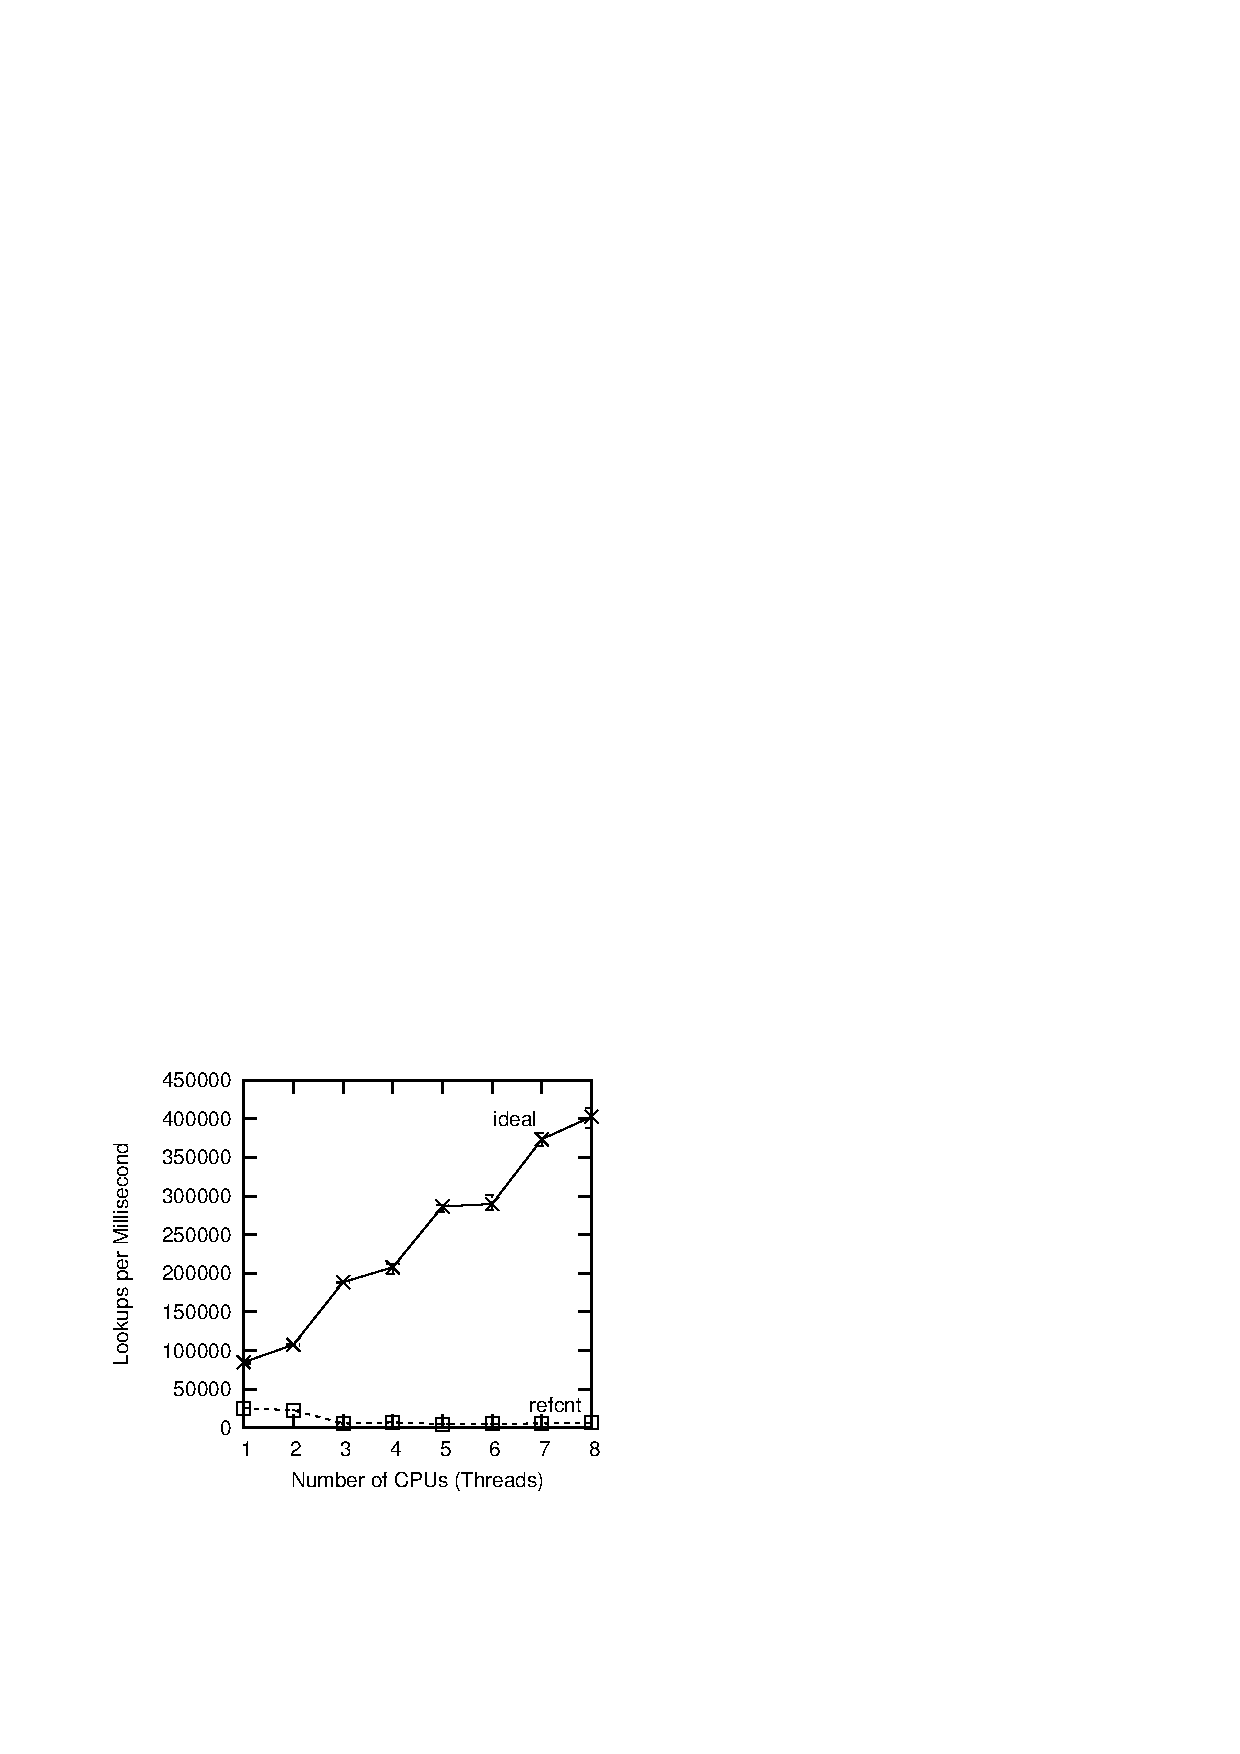
\includegraphics{CodeSamples/defer/perf-refcnt}}
\caption{Pre-BSD Routing Table Protected by Reference Counting}
\label{fig:defer:Pre-BSD Routing Table Protected by Reference Counting}
\end{figure}

Figure~\ref{fig:defer:Pre-BSD Routing Table Protected by Reference Counting}
는 싱글 소켓, 4 코어, 하이퍼쓰레드 가능한 2.5GHz x86 시스템에서 돌아가는 10개
원소 리스트에서의 read-only 워크로드가 레퍼런스 카운팅을 사용했을 때의 성능과
확장성을 보이고 있습니다.
``ideal'' 은
Listing~\ref{lst:defer:Sequential Pre-BSD Routing Table} 에서 보인, 이게 읽기만
하는 워크로드여서 동작할 수 있는 순차적 코드를
돌리는 것으로 만들어졌습니다.
``refcnt'' 선이 x~축에 붙어버리는 모습으로 볼 수 있듯 레퍼런스 카운팅 성능은
처참하고 그 확장성은 그보다도 더합니다.
Chapter~\ref{chp:Hardware and its Habits} 를 생각하면 이는 놀라운 일은
아닙니다:
레퍼런스 카운트 획득과 해제는 read-only 워크로드에서도 빈번한 공유 메모리
쓰기를 추가했고, 따라서 물리 법칙의 상당한 보복을 만들어냈습니다.
이 세상의 바람직한 생각은 최신 디지털 전자 기술에서 빛의 속도를 늘리거나 원자의
크기를 줄이는 것이 아님을 생각할 때 당연한 일입니다.
\iffalse

Figure~\ref{fig:defer:Pre-BSD Routing Table Protected by Reference Counting}
shows the performance and scalability of reference counting on a
read-only workload with a ten-element list running on a
single-socket four-core hyperthreaded 2.5\,GHz x86 system.
The ``ideal'' trace was generated by running the sequential code shown in
Listing~\ref{lst:defer:Sequential Pre-BSD Routing Table},
which works only because this is a read-only workload.
The reference-counting performance is abysmal and its scalability even
more so, with the ``refcnt'' trace dropping down onto the x-axis.
This should be no surprise in view of
Chapter~\ref{chp:Hardware and its Habits}:
The reference-count acquisitions and releases have added frequent
shared-memory writes to an otherwise read-only workload, thus
incurring severe retribution from the laws of physics.
As well it should, given that all the wishful thinking in the world
is not going to increase the speed of light or decrease the size of
the atoms used in modern digital electronics.
\fi

\QuickQuiz{}
	Figure~\ref{fig:defer:Pre-BSD Routing Table Protected by Reference Counting}
	에서 ``ideal'' 선은 왜 똑바로 증가하지 않고 계단 형태로 증가하죠?
	\iffalse

	Why the stairsteps in the ``ideal'' line in
	Figure~\ref{fig:defer:Pre-BSD Routing Table Protected by Reference Counting}?
	Shouldn't it be a straight line?
	\fi
\QuickQuizAnswer{
	하이퍼쓰레딩 때문입니다.
	이 시스템에서, 코어 위에서의 하드웨어 쓰레드들은 연속되는 CPU 번호를
	갖습니다.
	또한, 이 특정한 포인터를 따라가는, 낮은 캐시 미스 확률의 워크로드는
	하나의 하드웨어 쓰레드가 자신의 코어의 거의 모든 자원을 소모할 수
	있도록 하는 것으로 보입니다.
	더 많은 계산 작업을 갖는 워크로드는 각 코어의 두번째 하드웨어
	쓰레드로부터 더 많은 이득을 얻을 것이라 예상할 수 있을 겁니다.
	\iffalse

	The stair-steps are due to hyperthreading.
	On this particular system, the hardware threads in a given
	core have consecutive CPU numbers.
	In addition, this particular pointer-following
	low-cache-miss-rate workload seems
	to allow a single hardware thread to consume most of the
	relevant resources within its core.
	Workloads featuring heavier computational loads should be
	expected to gain greater benefit from each core's second
	hardware thread.
	\fi
} \QuickQuizEnd

\QuickQuiz{}
	요즘과 같은 시대에,
	Figure~\ref{fig:defer:Pre-BSD Routing Table Protected by Reference Counting}
	는 왜 겨우 8 CPU 까지만 사용하는 거죠???
	\iffalse

	Why, in these modern times, does
	Figure~\ref{fig:defer:Pre-BSD Routing Table Protected by Reference Counting}
	only go up to 8 CPUs???
	\fi
\QuickQuizAnswer{
	레퍼런스 카운팅의 끔찍한 확장성을 고려해보면, 누가 8개보다 많은 CPU 를
	필요로 하겠어요?
	CPU 네개까지만 해도 요점을 이야기 하는데 충분합니다!
	하지만, 더 많은 CPU 를 원하는 분들은
	Chapter~\ref{chp:Data Structures} 를 참고하시기 바랍니다.
	\iffalse

	Given the horrible scalability of reference counting, who needs
	more than eight CPUs?
	Four CPUs would have sufficed to make the point!
	However, people wanting more CPUs are urged to refer to
	Chapter~\ref{chp:Data Structures}.
	\fi
} \QuickQuizEnd

이게 끝이 아닙니다.

반복적으로 \co{route_add()} 와 \co{route_del()} 을 호출하는 여러개의 업데이트
쓰레드들을 수행시키게 되면
Listing~\ref{lst:defer:Reference-Counted Pre-BSD Routing Table Lookup} 의
line~37 의 해제 후 사용 버그를 알리는 \co{abort()} 문이 곧 수행될 겁니다.
이는 곧 레퍼런스 카운터가 확장성과 성능을 심각하게 저하시킬 뿐만 아니라, 필요한
보호를 제대로 제공하는데에도 실패함을 의미합니다.

Figure~\ref{fig:defer:Pre-BSD Packet Routing List} 에 보인 리스트에서 해제 후
사용 버그를 이끌어내는 이벤트 시퀀스 중 하나는 아래와 같습니다:
\iffalse

But it gets worse.

Running multiple updater threads repeatedly invoking
\co{route_add()} and \co{route_del()} will quickly encounter the
\co{abort()} statement on line~37 of
Listing~\ref{lst:defer:Reference-Counted Pre-BSD Routing Table Lookup},
which indicates a use-after-free bug.
This in turn means that the reference counts are not only profoundly
degrading scalability and performance, but also failing to provide
the needed protection.

One sequence of events leading to the use-after-free bug is as follows,
given the list shown in
Figure~\ref{fig:defer:Pre-BSD Packet Routing List}:
\fi

\begin{enumerate}
\item	Thread~A 가 address~42 를 탐색해서
	Listing~\ref{lst:defer:Reference-Counted Pre-BSD Routing Table Lookup}
	\co{route_lookup()} 의 line~33 에 도달합니다.
	달리 말해, Thread~A 는 첫번째 원소로의 포인터를 갖고 있지만, 아직
	그로의 레퍼런스를 획득하진 못한 상태입니다.
\item	Thread~B 가 address~42 의 route 원소를 지우려고
	Listing~\ref{lst:defer:Reference-Counted Pre-BSD Routing Table Add/Delete}
	의 \co{route_del()} 을 호출합니다.
	이는 성공적으로 완료되며, 이 원소의 \co{->re_refcnt} 필드는 그 값이
	1이므로, \co{->re_freed} 필드를 설정하고 원소를 해제하기 위해
	\co{re_free()} 를 호출합니다.
\item	Thread~A 는 \co{route_lookup()} 의 수행을 계속합니다.
	\co{rep} 로의 포인터는 \co{NULL} 이 아니지만, line~36 은 자신의
	\co{->re_freed} 필드가 0이 아님을 보게 되어서 line~37 에서 \co{abort()}
	를 호출하게 됩니다.
\iffalse

\item	Thread~A looks up address~42, reaching line~33 of
	\co{route_lookup()} in
	Listing~\ref{lst:defer:Reference-Counted Pre-BSD Routing Table Lookup}.
	In other words, Thread~A has a pointer to the first element,
	but has not yet acquired a reference to it.
\item	Thread~B invokes \co{route_del()} in
	Listing~\ref{lst:defer:Reference-Counted Pre-BSD Routing Table Add/Delete}
	to delete the route entry for address~42.
	It completes successfully, and because this entry's \co{->re_refcnt}
	field was equal to the value one, it invokes
	\co{re_free()} to set the \co{->re_freed} field and to free the entry.
\item	Thread~A continues execution of \co{route_lookup()}.
	Its \co{rep} pointer is non-\co{NULL}, but line~36 sees that
	its \co{->re_freed} field is non-zero, so line~37 invokes
	\co{abort()}.
\fi
\end{enumerate}

문제는 이 레퍼런스 카운트가 보호되어야 할 오브젝트 안에 위치해 있다는 것인데,
이는 레퍼런스 카운트 자체가 획득되는 시점에서는 어떤 보호도 없음을 의미합니다!
이는 Gamsa 등~\cite{Gamsa99} 에 의해 이야기되었던 락킹에서의 문제의 레퍼런스
카운팅에서의 비슷한 경우입니다.
Route 원소별로 레퍼런스 카운트 획득을 보호하기 위한 글로벌 락이나 레퍼런스
카운트를 생각해 볼 수도 있겠지만, 이는 상당한 경쟁 문제를 초래할 수 있습니다.
동시성 있는 환경에서 안전한 레퍼런스 카운트 획득을 위한 알고리즘들이 존재하긴
합니다만~\cite{Valois95a}, 그것들은 굉장히 복잡할 뿐더러 에러를 만들기가
쉬운데다가~\cite{MagedMichael95a} 처참한 성능과 확장성을
제공합니다~\cite{ThomasEHart2007a}.

한마디로, 동시성은 분명히 레퍼런스 카운팅의 유용성을 저하시켰습니다!
\iffalse

The problem is that the reference count is located in the object
to be protected, but that means that there is no protection during
the instant in time when the reference count itself is being acquired!
This is the reference-counting counterpart of a locking issue noted
by Gamsa et al.~\cite{Gamsa99}.
One could imagine using a global lock or reference count to protect
the per-route-entry reference-count acquisition, but this would
result in severe contention issues.
Although algorithms exist that allow safe reference-count acquisition
in a concurrent environment~\cite{Valois95a}, they are not only extremely
complex and error-prone~\cite{MagedMichael95a}, but also provide
terrible performance and scalability~\cite{ThomasEHart2007a}.

In short, concurrency has most definitely reduced the usefulness
of reference counting!
\fi

\QuickQuiz{}
	동시성이 ``분명히 레퍼런스 카운팅의 유용성을 저하시켰다''면, 리눅스
	커널은 왜 그렇게 레퍼런스 카운터를 많이 사용하는거죠?
	\iffalse

	If concurrency has ``most definitely reduced the usefulness
	of reference counting'', why are there so many reference
	counters in the Linux kernel?
	\fi
\QuickQuizAnswer{
	그 문장은 ``유용성을 저하시켰다'' 고 했지, ``유용성을 없앴다'' 고는
	하지 않았습니다, 그렇죠?

	리눅스 커널이 레퍼런스 카운팅의 장점을 높은 동시성이 존재하는 환경에서
	가져오기 위해 사용하는 방법들을 이야기하는
	Section~\ref{sec:together:Refurbish Reference Counting} 를 보기
	바랍니다.
	\iffalse

	That sentence did say ``reduced the usefulness'', not
	``eliminated the usefulness'', now didn't it?

	Please see
	Section~\ref{sec:together:Refurbish Reference Counting},
	which discusses some of the techniques that the Linux kernel
	uses to take advantage of reference counting in a highly
	concurrent environment.
	\fi
} \QuickQuizEnd

그렇다곤 하지만, 가끔은 문제를 해결하기 위해선 완전히 다른 방법으로 문제를
바라볼 필요가 있습니다.
다음 섹션에서는 상당한 성능과 확장성을 제공하는, 안에서 바깥으로의 레퍼런스
카운트에서 생각해 볼수 있는 것들을 논해 봅니다.
\iffalse

That said, sometimes it is necessary to look at a problem in an
entirely different way in order to successfully solve it.
The next section describes what could be thought of as an
inside-out reference count that provides decent performance
and scalability.
\fi
